\section{Inner Product Spaces}
\subsubsection*{Motivation}
\begin{definition}
    In $\b R^n$, the dot product of $\vec x$ and $\vec y$ is defined by  
\[ \vec x \cdot \vec y := x_1y_1 + x_2y_2 + \cdots + x_ny_n\]
for $\vec x = (\li xn), \vec y = (\li yn)$.
\end{definition}
\subsection{Inner Product and Norms}
\subsubsection*{Settings}
$V$ is a vector space over $\b F$, we can define the following mapping $ \la \cdot, \cdot \ra : V \times V \to \b F$.
\begin{definition}
$\la \cdot, \cdot \ra$ is called an inner product if it satisfying the following rules:
\begin{enumerate}
    \item(additivity in the first slot) $\la \vec v + \vec u, \vec w \ra = \la \vec v + \vec w \ra + \la \vec u, \vec w \ra, \ \forall \vec v, \vec u, \vec w \in V$
    \item(homogeneity in the first slot) $\la \lambda \vec v, \vec w \ra = \lambda \la \vec v + \vec w \ra, \ \forall \vec v \vec u, \vec w \in V, \lambda \in \b F$
    \item(conjugate symmetry) $\la \vec v, \vec w \ra = \overline{\la \vec w, \vec v \ra}, \ \forall \vec v,\vec w \in V$
    \item(positivity) $\la \vec v, \vec v \ra \geq 0, \ \forall \vec v \in V$
    \item(definiteness) $\la \vec v, \vec v \ra = 0$ iff $\vec v = \vec 0$.
\end{enumerate}
\end{definition}
\begin{question}
What about linearity in the second slot?
\end{question}
\begin{answer} We can compute
\[ \la \vec v, \vec u + \vec w \ra = \overline{\la \vec u + \vec w, \vec v\ra} = \overline{\la \vec u, \vec v \ra + \ra \vec w, \vec v} = \overline{\la \vec u, \vec v \ra} + \overline{\la \vec w, \vec v\ra } = \la \vec v, \vec u\ra + \la \vec v, \vec w\ra\]
\[ \la \vec v, \lambda \vec u\ra = \overline{\la \lambda u, \vec v\ra} = \overline{\lambda \la \vec u,\vec v\ra} = \bar \lambda \ \overline{\la \vec u, \vec v\ra} = \bar \lambda \la \vec v, \vec u \ra\]
Not quite. \frownie{}
\end{answer}
\begin{remark}
    If $\vec v \in V$ is fixed then the function $\la \cdot, \vec v \ra : \vec u \mapsto \la \vec u, \vec v \ra$ is a function functional. 
\end{remark}
\begin{example}
    On $\b R^n$, we could use any function of the type
    \[ c_1x_1y_1 + c_2x_2y_2 + \cdots + c_nx_ny_n\] where all $c_j \in \b R^+$.
\end{example}
\begin{remark}[Generalization to $\b C^n$]
    The inner product of this form of the standard product to $\b C^n$ can be defined as
    \[ \la \vec x, \vec y \ra = x_1\bar y_1 + x_2\bar y_2 + \cdots + x_n\bar y_n\]
\end{remark}
\begin{remark}[Generalization to any function space]
    \[ \la f, g \ra : = \int_D f(t)\overline{g(t)} dt\]
    or generally \[ \la f, g \ra : = \int_D f(t)\overline{g(t)}w(t) dt\]
    where $w(t)$ is the positive weight function. e.g. if $V = \c P(\b R)$, or $V = \c P(\b C)$, then 
    \[ \la f, g \ra : = \int_0^\infty f(t)\overline{g(t)}e^{-t} dt\]
\end{remark}
\begin{definition}
    For $v \in V$, the (Euclidean) Norm is defined as
    \[ ||v|| : = \sqrt{\la v,v \ra}\] 
\end{definition}
\begin{theorem}(Properties of Norms)
    \begin{enumerate}
        \item $||\lambda v || = |\lambda| \ ||v|| \ \forall v \in V, \forall \lambda \in \b F $
        \item $||v|| > 0$ for all $v \in V$
        \item $||v|| = 0$ if and only if $v = 0$ 
    \end{enumerate}
\end{theorem}
\begin{definition}
    An inner product space is a vector space $V$ along with and inner product on $V$.
\end{definition}
\begin{definition}
    For $u,v \in V$, we say $u$ and $v$ is orthogonal if $\la u, v\ra = 0$
\end{definition}
\begin{theorem}[Pythagorean Theorem] $ $
\begin{center}
    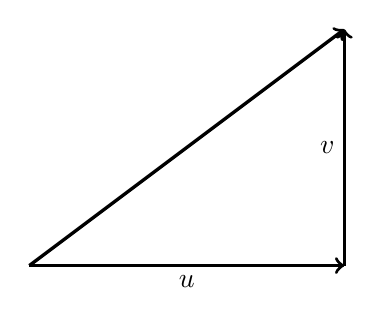
\begin{tikzpicture}
        \draw[->, very thick] (4,0) -- (4,3);
        \draw[->, very thick] (0,0) -- (4,0);
        \draw[->, very thick] (0,0) -- (4,3);
        \draw (2,0) node[anchor = north] {$u$};
        \draw (4,1.5) node[anchor = east] {$v$};
    \end{tikzpicture}
\end{center}
\[ ||u + v||^2 = ||u||^2 + ||v||^2 \iff \la u + v, u + v\ra = \la u,u \ra + \la v,v \ra \]
\end{theorem}
\begin{proof} We compute
    \[ \la u + v, u + v\ra = \la u,u \ra + \la u , v \ra + \la v, u \ra + \la v,v \ra = \la u,u \ra + 0 + 0 + \la v,v \ra = ||u|| + ||v|| \]
\end{proof}
\subsubsection*{Obeservation}
Given $u,v \in V$ such that $v \neq 0$, we want to modify $u$ such that $u + cv$ is orthogonal to $v$. We know that $\la v + cv, v \ra = 0$, solve for $c$ gives $c = \displaystyle\frac{-\la u, v\ra}{\la v, v \ra}$.
\begin{center}
    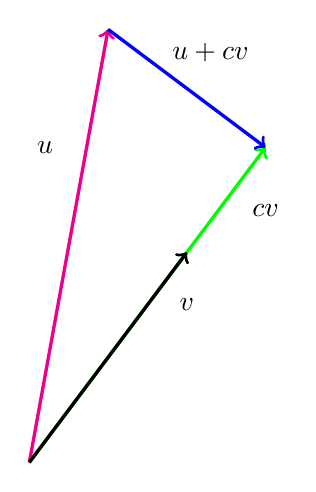
\begin{tikzpicture}
        \draw[->, very thick, color = magenta] (0,0) -- (1, 5.5);
        \draw[->, very thick, color = green] (0,0) -- (3, 4);
        \draw[->, very thick] (0,0) -- (2,2.66666666);
        \draw[->, very thick, color = blue] (1, 5.5) -- (3,4);
        \draw (2,2) node {$v$};
        \draw (0.2,4) node {$u$};
        \draw (3,3.2) node {$cv$};
        \draw (2.3, 5.2) node {$u + cv$};
    \end{tikzpicture} 

    An orthogonal decompostion
\end{center}
\begin{theorem}[Cauchy-Schwarz Inequality]
    For any $u,v \in V$ where $V$ is a inner product space, the following holds
    \[ |\la u,v \ra| \leq ||u|| \cdot ||v||\]
\end{theorem}
\begin{proof}
    Given $u,v \in V$, we can assume without the loss of generality that $v \neq 0$. So we can consider vectors $u + cv$ and $v$ that are orthogonal for the choice that 
    \[ c: = \frac{ - \la u,v \ra}{\la v,v\ra}\]
    By Pathgrathrean theorem, $||u + cv||^2 + ||cv||^2 = ||u||^2$. But $||cv||^2 = |c|^2||v||^2$ and recall \[ c= \frac{- \la u,v\ra}{\la v,v\ra}, \text{ so } c^2= \frac{|\la u,v\ra|^2}{\la v,v\ra^2} = \frac{|\la u, v \ra|^2}{||v||^4}, \text{ therefore } ||cv||^2 = \frac{|\la u, v \ra|^2}{||v||^4} ||v||^2 = \frac{|\la u, v \ra|^2}{||v||^2}\]
    So by dropping $|| u + cv||^2 > 0$, we obtain $||cv||^2 \leq ||u||$, i.e, 
    \[ \frac{|\la u, v \ra|^2}{||v||^2} \leq ||u||^2 \implies |\la u,v\ra|^2 \leq ||u|^2 \cdot ||v||^2 \implies |\la u,v \ra|^2 \leq ||u|| \cdot ||v||\]
\end{proof}


